\documentclass[10pt,journal,compsoc]{IEEEtran}

\usepackage{algorithmic}
\usepackage{array}
 \usepackage[nocompress]{cite}
 \usepackage{color}
\usepackage{listings}
\usepackage[caption=false,font=normalsize,labelfont=sf,textfont=sf]{subfig}
\usepackage{stfloats}
\usepackage{url}


\usepackage[pdftex]{graphicx}
\graphicspath{{./figs}}
\DeclareGraphicsExtensions{.pdf,.jpeg,.png}


% *** MATH PACKAGES ***
\usepackage{amsmath}
\interdisplaylinepenalty=2500

% correct bad hyphenation here
\hyphenation{op-tical net-works semi-conduc-tor}


\begin{document}

% title
\title{Reproducible Workflow on a Public Cloud for Computational Fluid Dynamics}
% author names and affiliations
\author{Olivier Mesnard, Lorena A. Barba
\IEEEcompsocitemizethanks{\IEEEcompsocthanksitem Mechanical and Aerospace Engineering,
the George Washington University, Washington, DC 20052.\protect\\
% note need leading \protect in front of \\ to get a newline within \thanks as
% \\ is fragile and will error, could use \hfil\break instead.
E-mail: mesnardo@gwu.edu
\IEEEcompsocthanksitem Email: labarba@gwu.edu}% <-this % stops an unwanted space
%\thanks{Manuscript submitted 2019}
}

\IEEEtitleabstractindextext{%
\begin{abstract}
In a new effort to make our research transparent and reproducible by others, we have developed a workflow to run computational studies on a public cloud. It uses Docker containers to create an image of the application software stack. We also adopt several tools that facilitate creating and managing virtual machines with compute nodes and submitting jobs to these nodes. The configuration files for these tools are part of an expanded "reproducibility package" that includes workflow definitions for cloud computing, in addition to input files and instructions. This facilitates re-creating the cloud environment to re-un the simulations under the same conditions.
\end{abstract}
}

% make the title area
\maketitle

\IEEEraisesectionheading{\section{Introduction}\label{sec:introduction}}

\section{Reproducible Workflow}\label{sec:workflow}

CFD publications often lack details about external libraries used along with the main computational code.
We have learned the hard way how different versions of the same external library can alter the numerical results and even the scientific findings of a computational study\cite{mesnard_barba_2017}.
To overcome the so-called ``dependency hell'' and facilitate reproducibility, we use Docker to locally create an image of our computational application.
Container technology facilitates share build images of the full software stack that is used to produce scientific results.
The process of building an image using Docker begins with writing an ASCII file, called a Dockerfile, that contains Docker keywords and system commands for building multi-layered software stack.
Once the image is build locally, we push it to a public registry (e.g., DockerHub).
Everyone can now pull the application image and create a container to run the application in a faithfully reproduced local environment.
We aim to move the final stage of this workflow (creating a container) to a public cloud provider such as Microsoft Azure.

To run computational jobs on Microsoft Azure, we use several tools that facilitate creating and managing virtual machines with compute nodes and submitting jobs to those nodes.
\ref{fig:cloud_workflow} shows a graphical representation of the workflow we adopted to run CFD simulations with an in-house software on Microsoft Azure.

\begin{figure}[!ht]
    \centering
    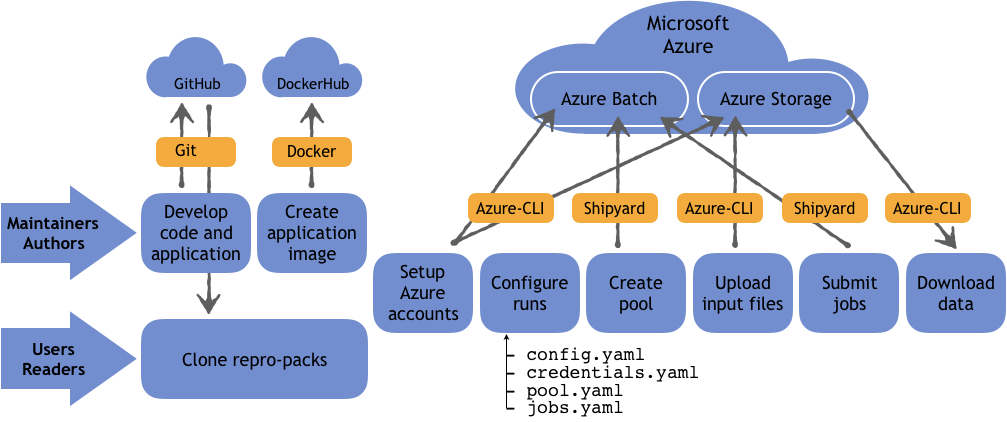
\includegraphics[width=7cm]{figures/cloud_workflow.png}
    \caption{Reproducible workflow on the public cloud provider Microsoft Azure.}
    \label{fig:cloud_workflow}
\end{figure}

\begin{table}[!t]
    \caption{NC series on Microsoft Azure. (Prices as of May 13, 2018.)}
    \label{tab:nc_series}
    \centering
    \begin{tabular}{cccccccc}
        Instance & cores & RAM (GiB) & disk sizes (GiB) & GPU & pay-as-you-go (\$/hr) & 1-year reserved (\$/hr) & 3-year reserved (\$/hr) \\
        \hline
        NC6 & 6 & 56 & 340 & 1 x K80 & 0.90 & 0.574 & 0.40 \\
        NC12 & 12 & 112 & 680 & 2 x K80 & 1.80 & 1.147 & 0.80 \\
        NC24 & 24 & 224 & 1,440 & 4 x K80 & 3.60 & 2.294 & 1.599 \\
        NC24r$^\dagger$ & 24 & 224 & 1,440 & 4 x K80 & 3.96 & 2.523 & 1.758 \\
        \hline
    \end{tabular}
    $\dagger$ NC24r: RDMA (Remote Direct Access Memory) capable with InfiniBand network.
\end{table}

\section{Results}\label{sec:results}

\subsection{MPI Communication Benchmarks}\label{subsec:mpi_benchmarks}

\begin{figure}[!ht]
    \centering
    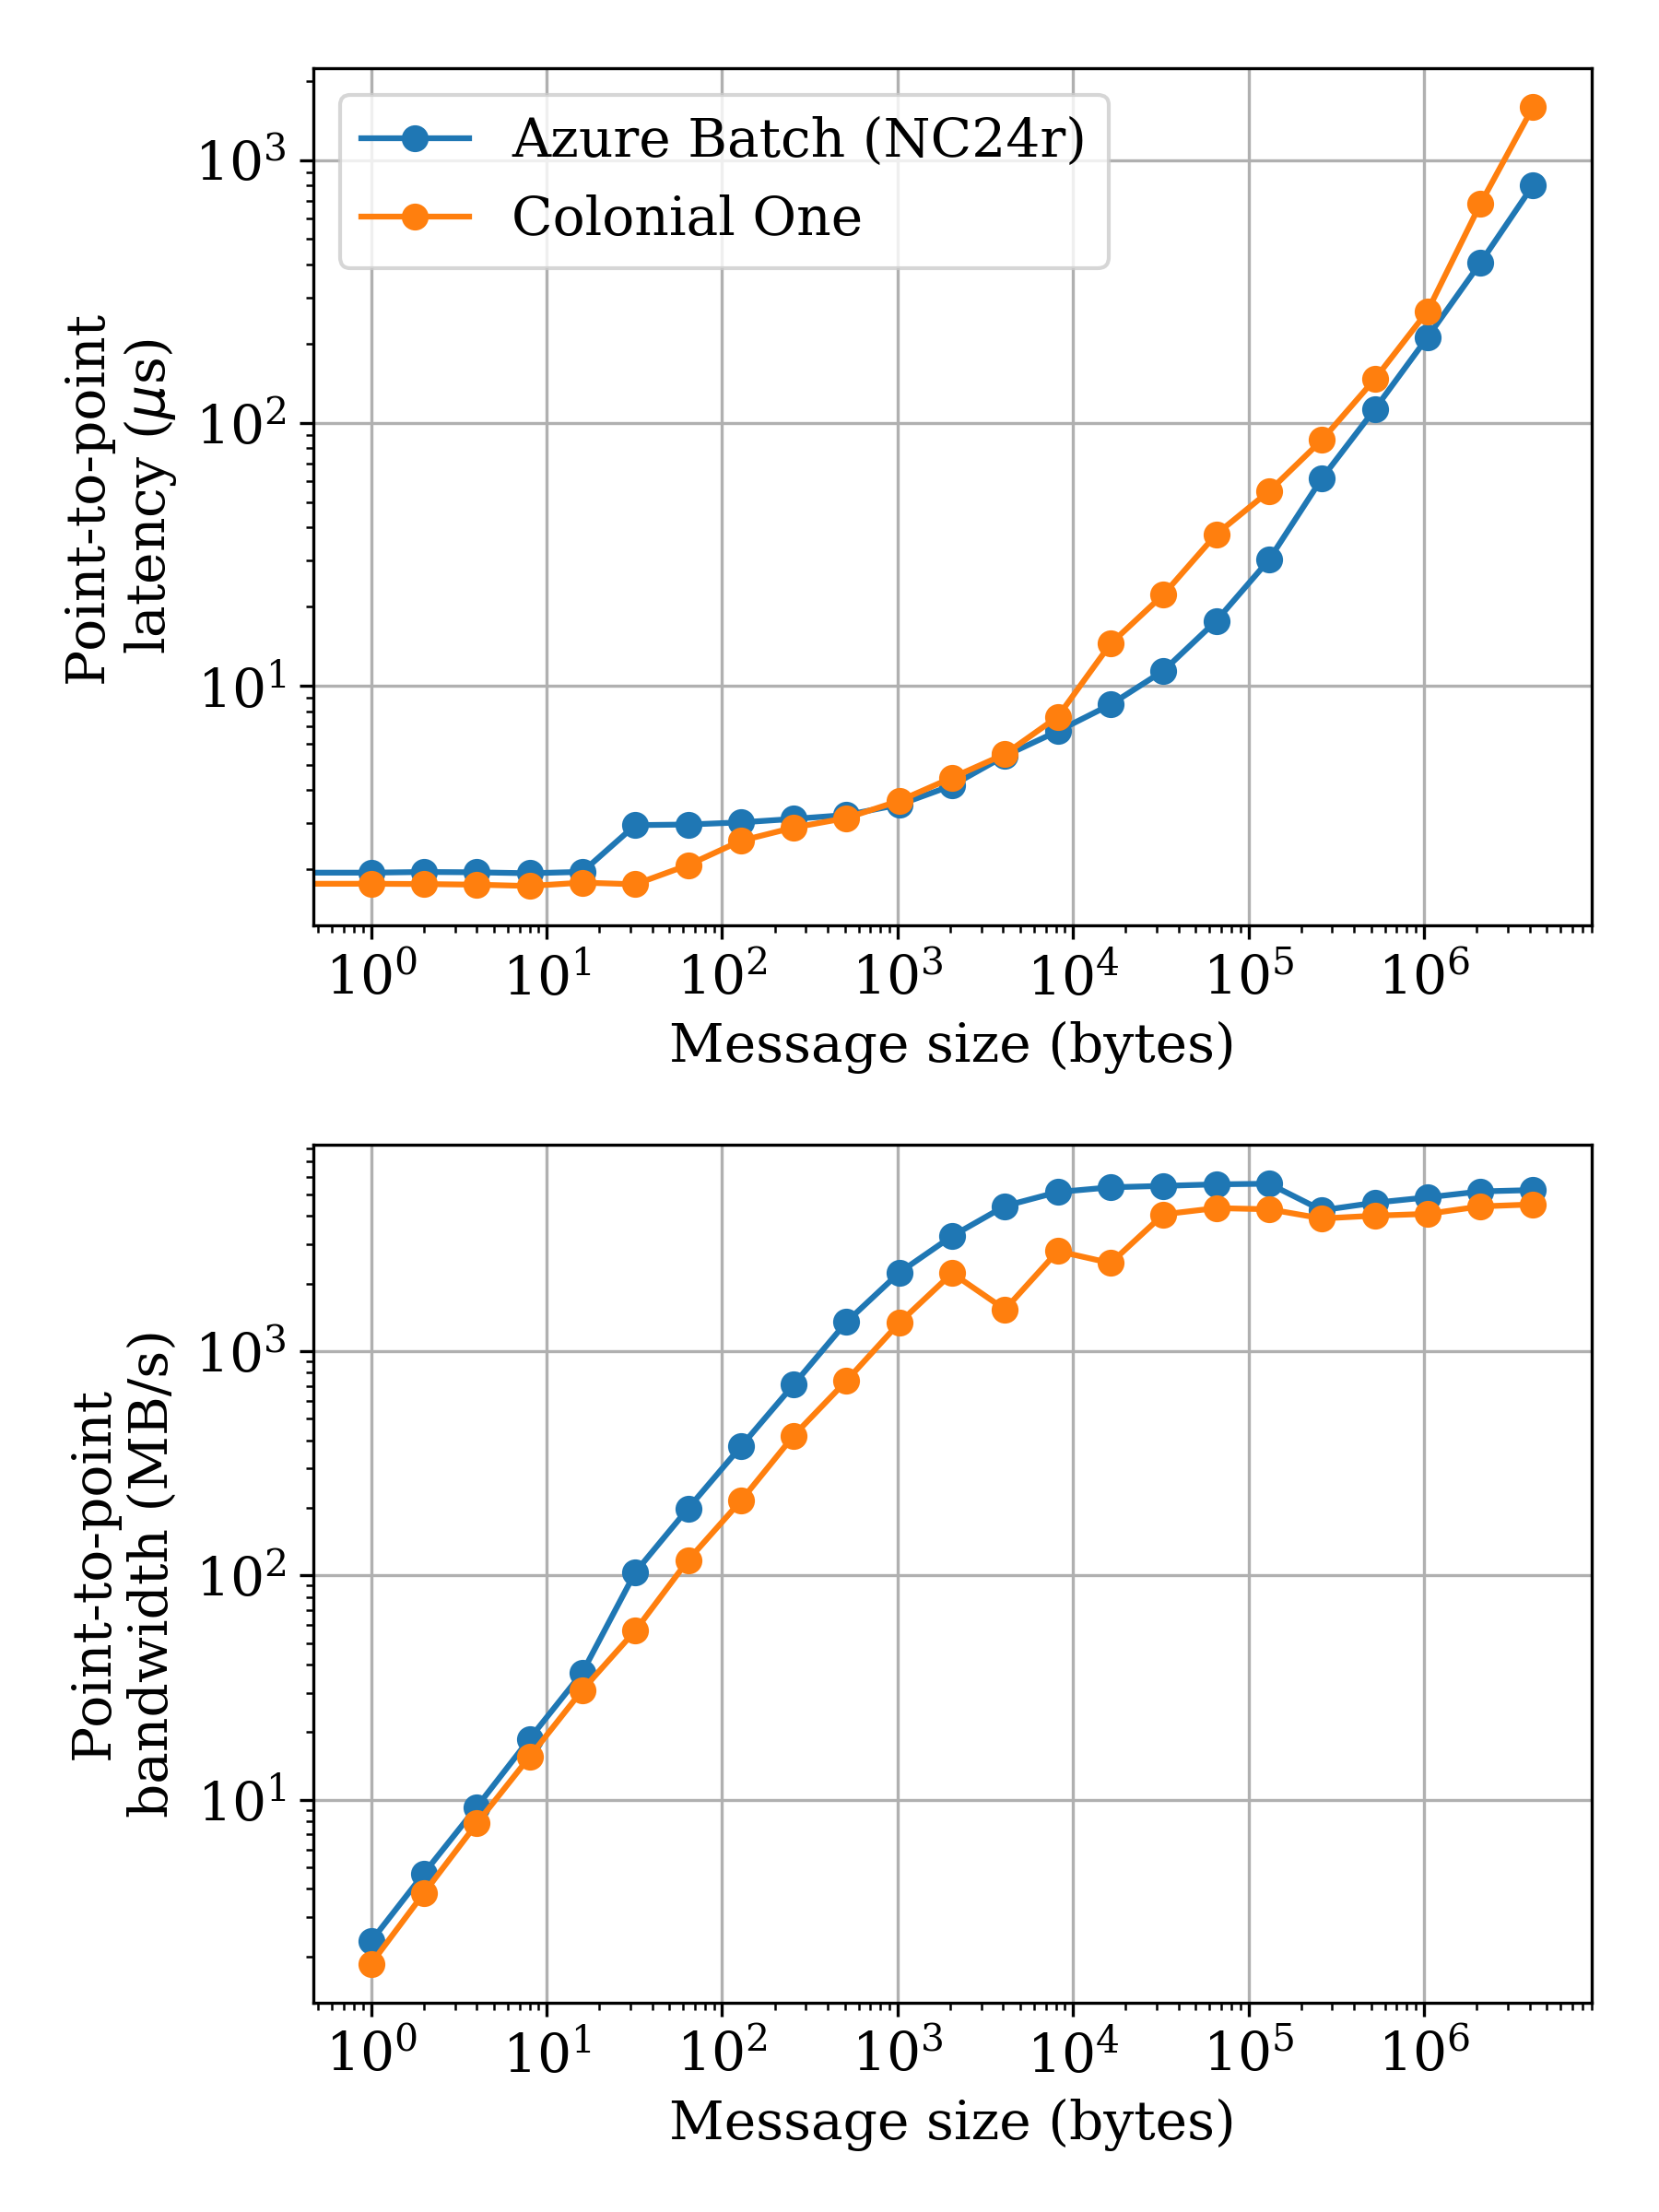
\includegraphics[width=7cm]{figures/osu_latency_bandwidth.png}
    \caption{Point-to-point latency (top) and bandwidth (bottom) obtained on Colonial One and on NC24r instances of Microsoft Azure.}
    \label{fig:osu_benchmarks}
\end{figure}

\subsection{Poisson Benchmarks}\label{subsec:poisson_benchmarks}

\begin{figure}[!ht]
    \centering
    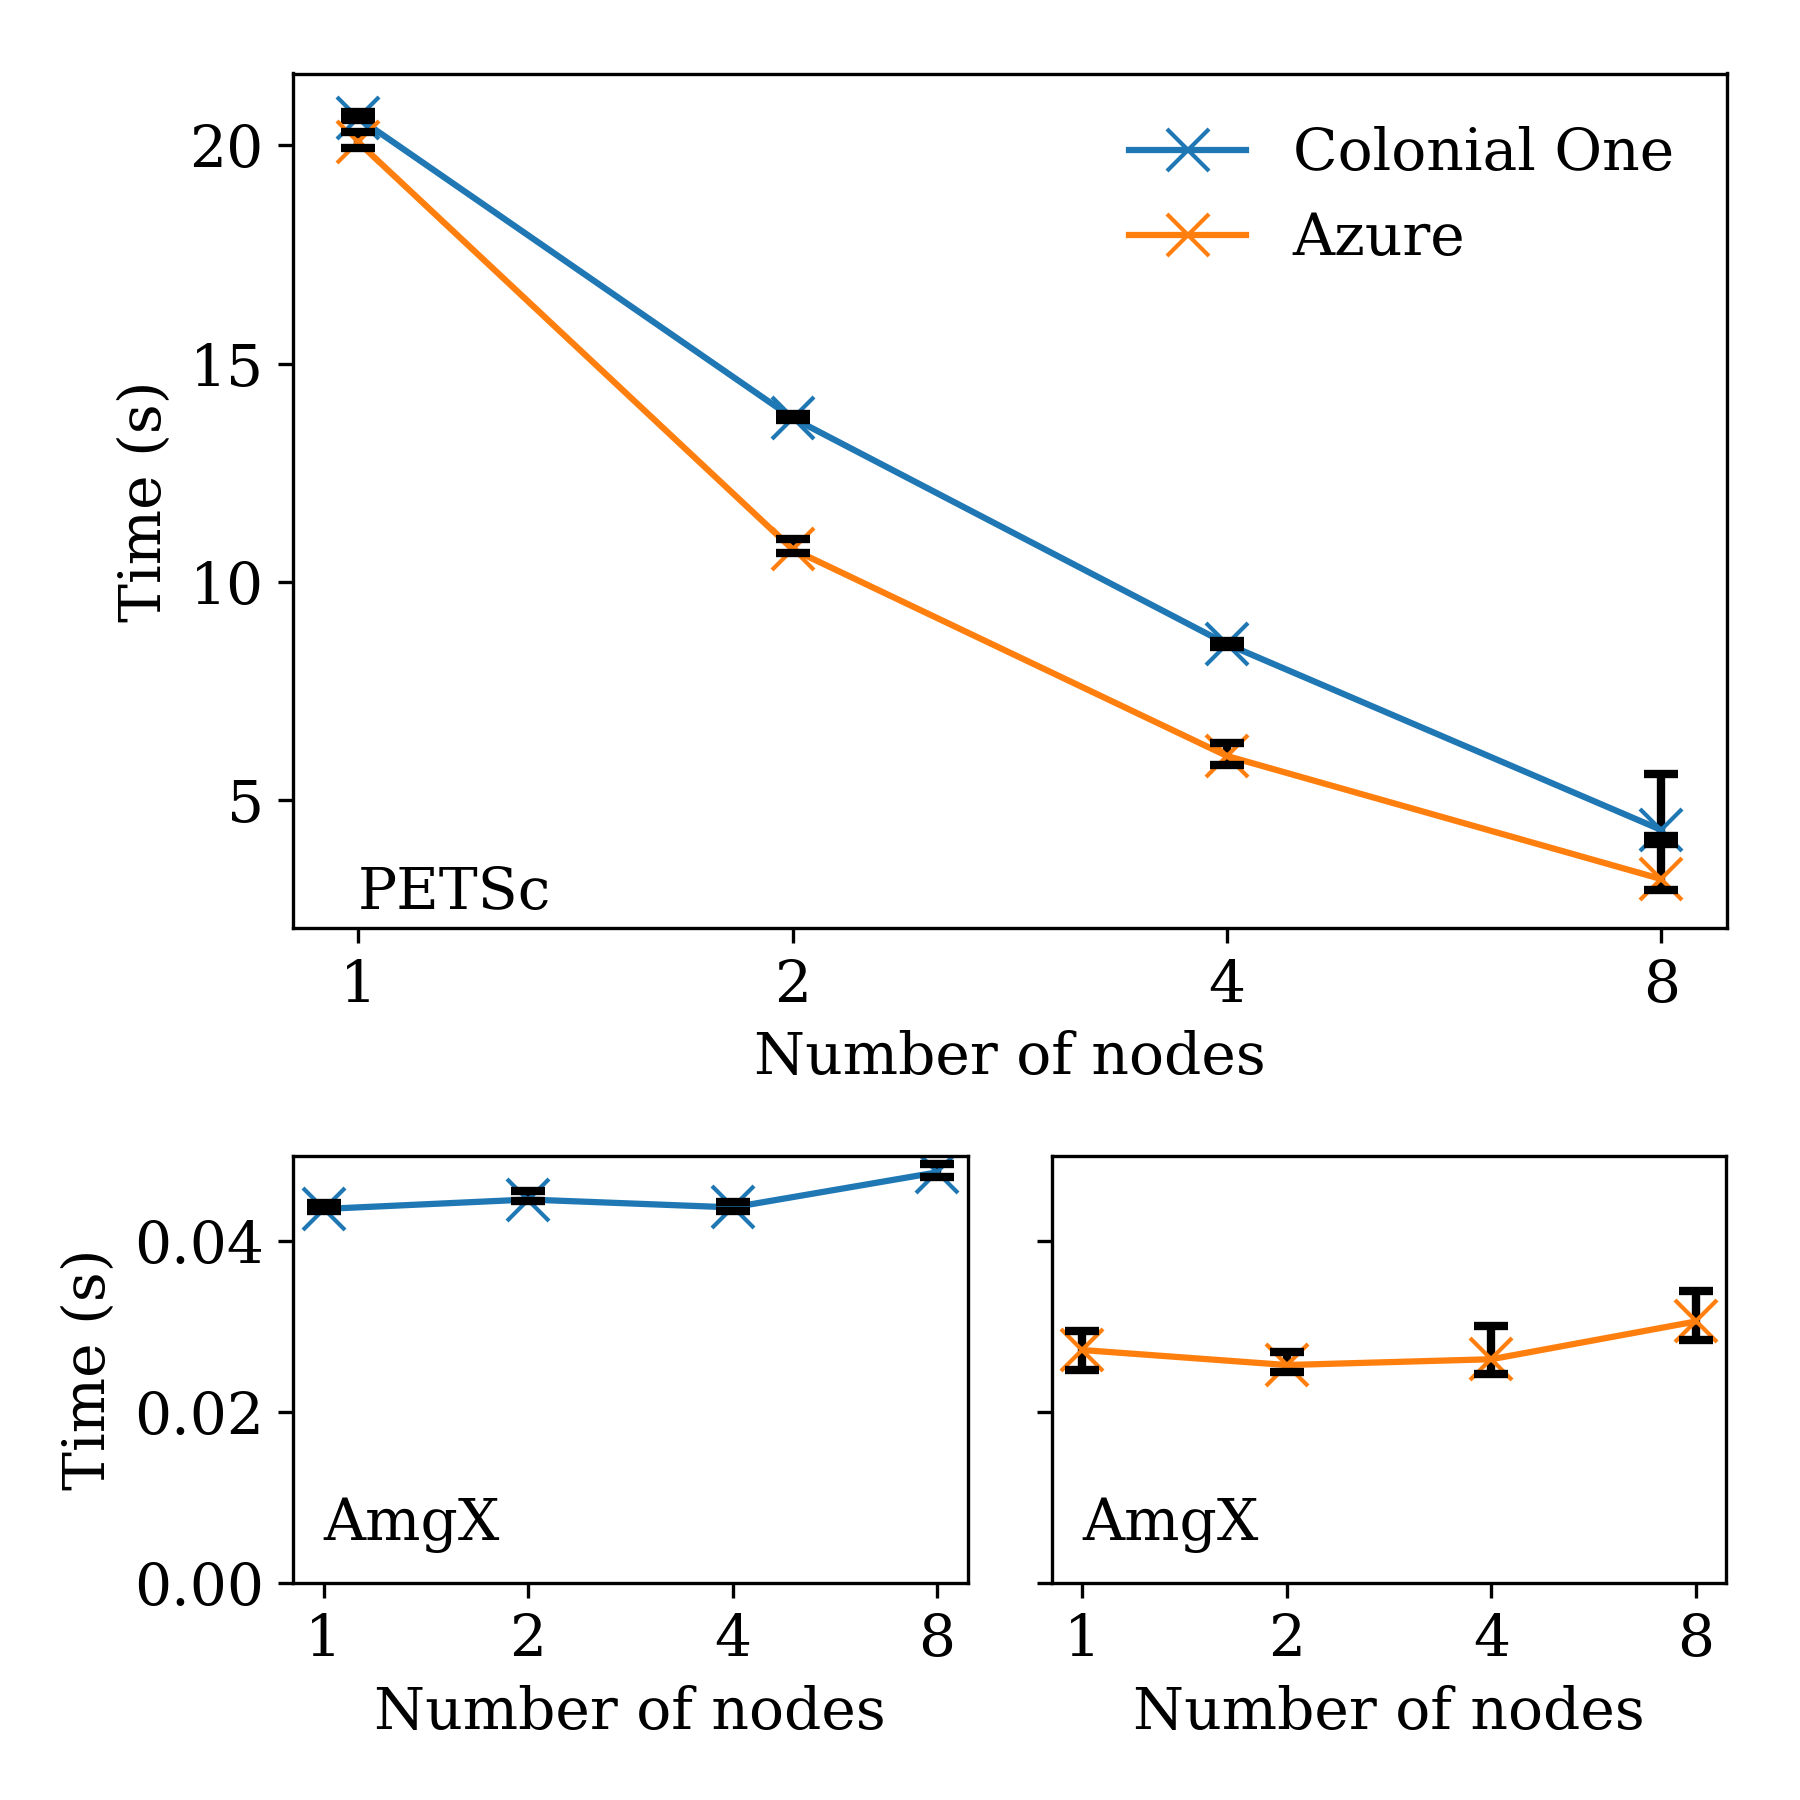
\includegraphics[width=7cm]{figures/poisson_time_vs_nodes.png}
    \caption{Runtimes to solve a Poisson system on Colonial One and on Microsoft Azure.}
    \label{fig:poisson_benchmarks}
\end{figure}

\subsection{Flow Around a Flying Snake Cross-Section}\label{subsec:snake}

Our research lab is interested in understanding the aerodynamics of flying animals using Computational Fluid Dynamics software.
One of our applications deals with the aerodynamics of a snake species, \textit{Chrysopelea Paradisi}, that lives in South-East Asia.
The arboreal reptile has the remarkable capacity to turn its entire body into a wing and glide over several meters\cite{socha_2011}.
The so-called flying snake jumps from tree branches, undulates in the air, and is able to produce lift by expanding its ribcage to flatten its ventral surface (morphing its normally circular cross-section into a triangular shape).

\begin{figure}[!ht]
    \centering
    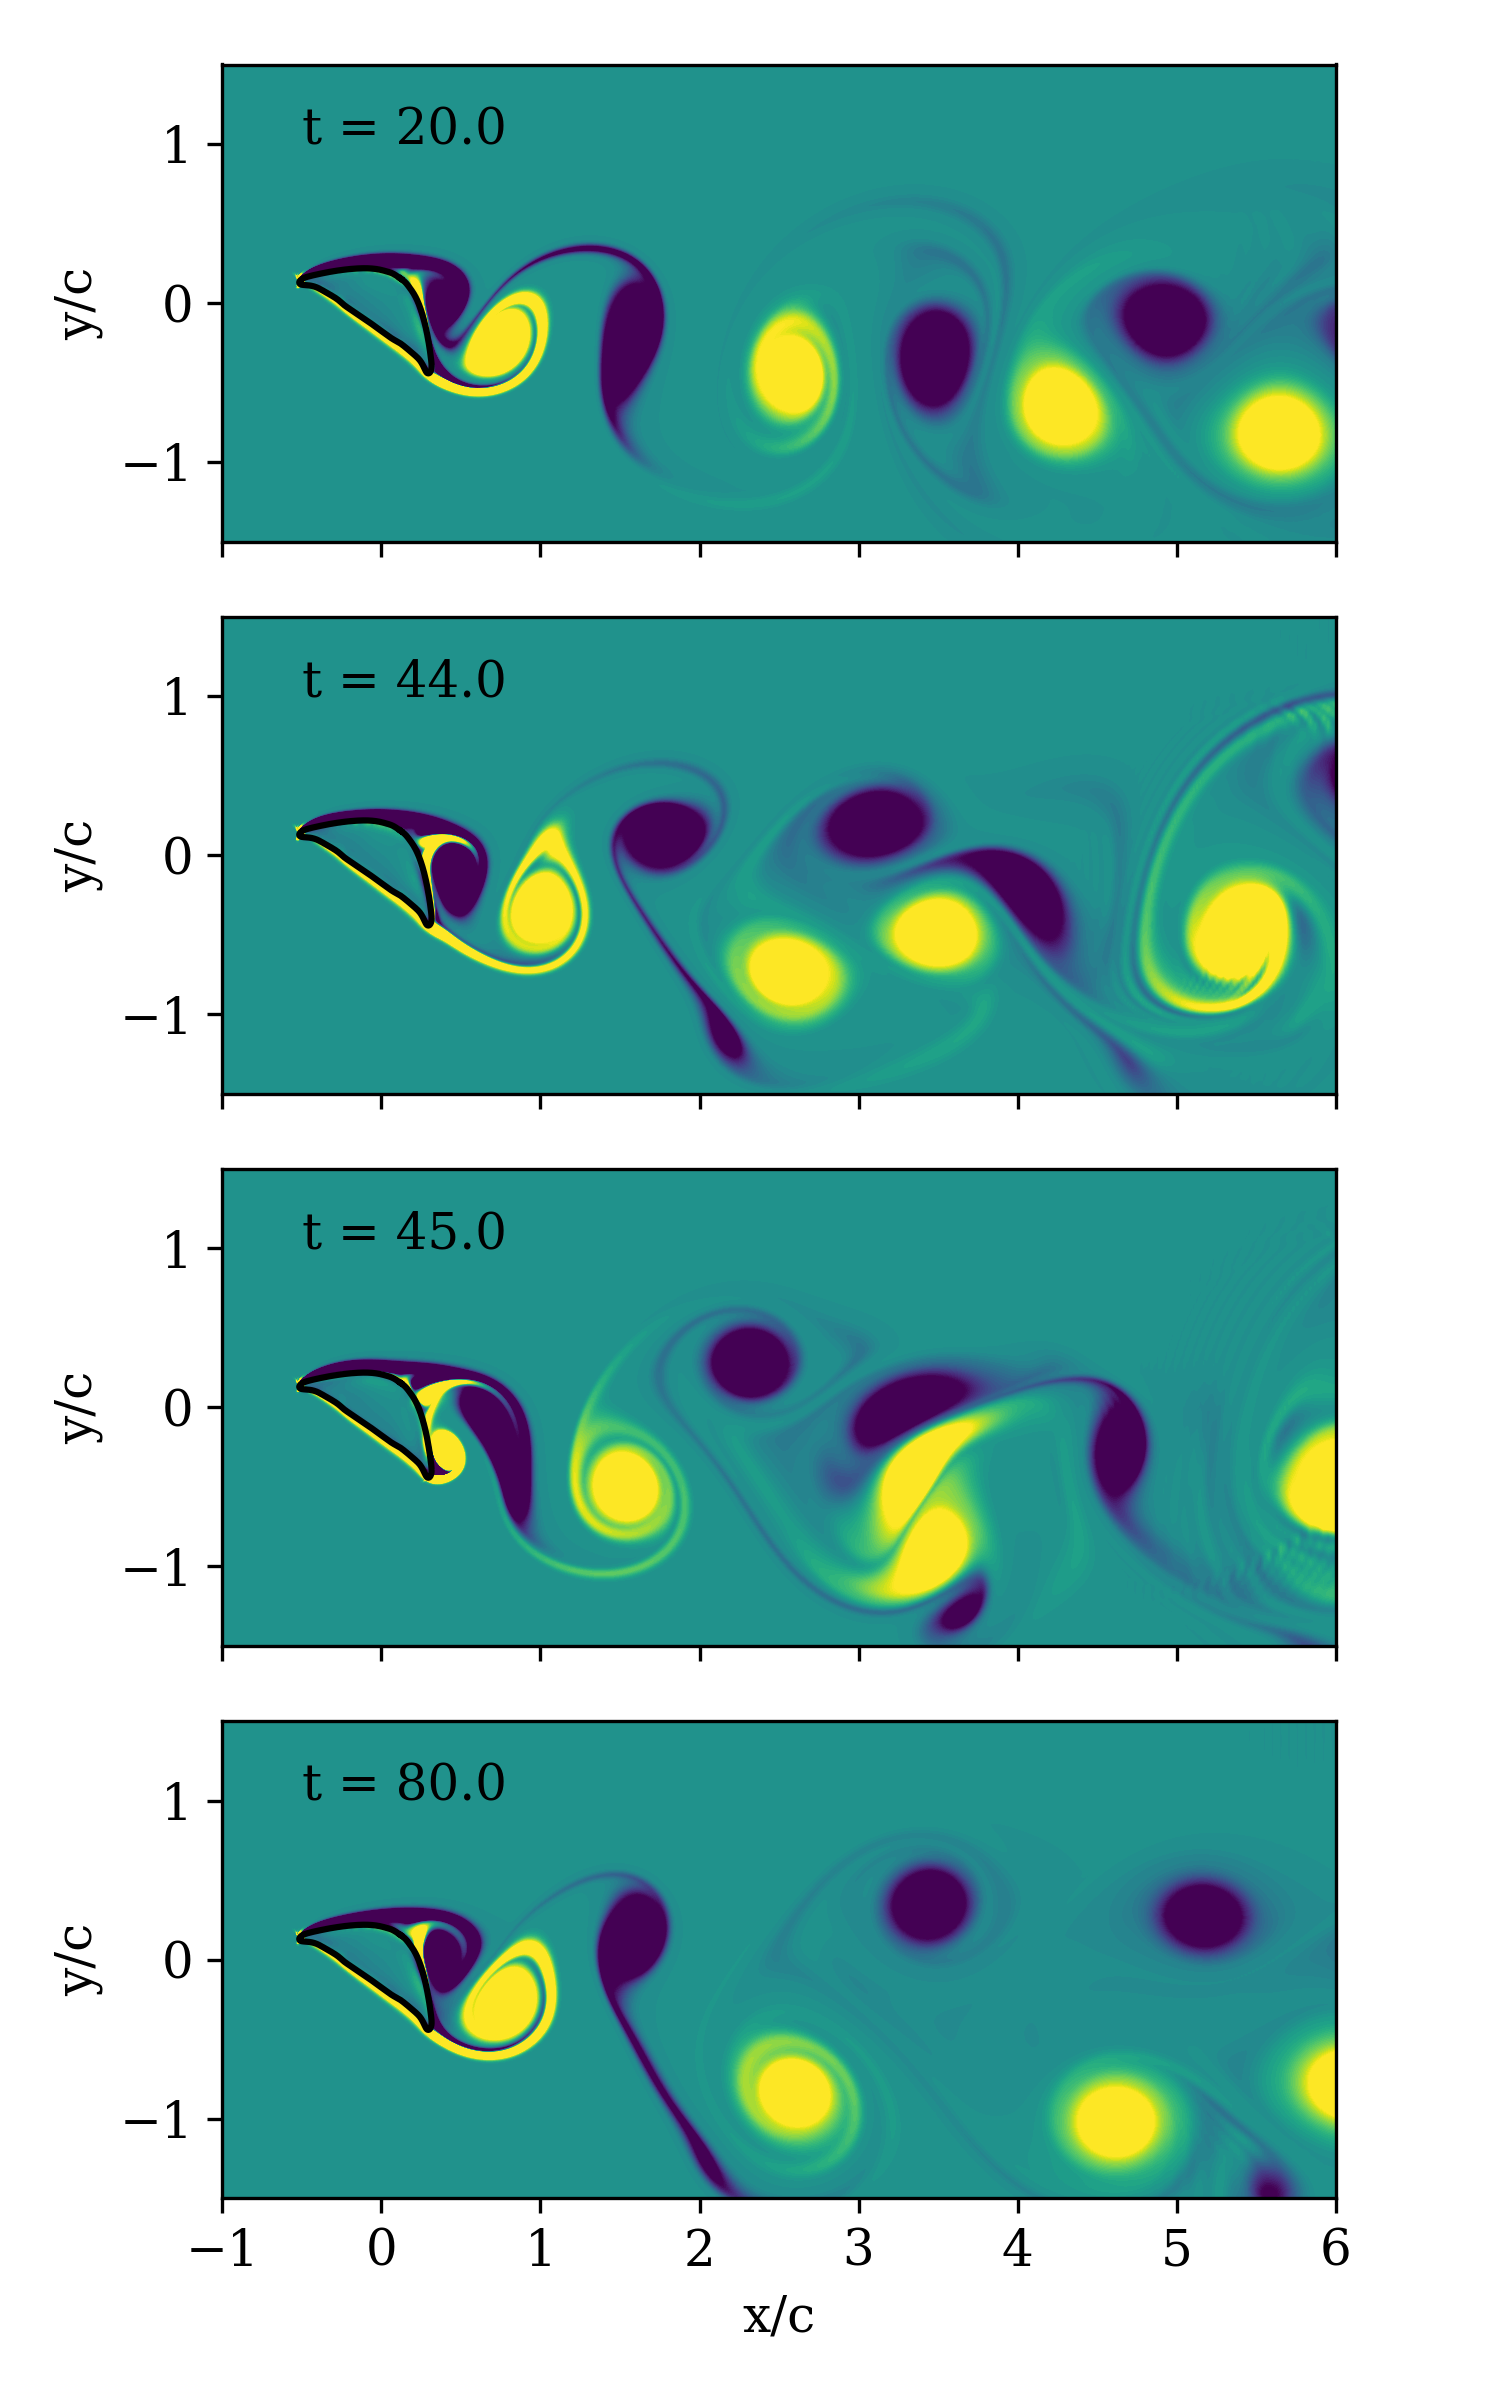
\includegraphics[width=7cm]{figures/wz_multi_contourf.png}
    \caption{Filled contour of the vorticity field after $20$, $44$, $45$, and $80$ time units fo flow simulation with PetIBM for the snake cross-section at a $35$-degree angle of attack and Reynolds number $2000$. Vortex merging events are responsible for the change in the wake signature and the drop in the mean value of the lift coefficient.}
    \label{fig:vorticity2d}
\end{figure}

\begin{figure}[!ht]
    \centering
    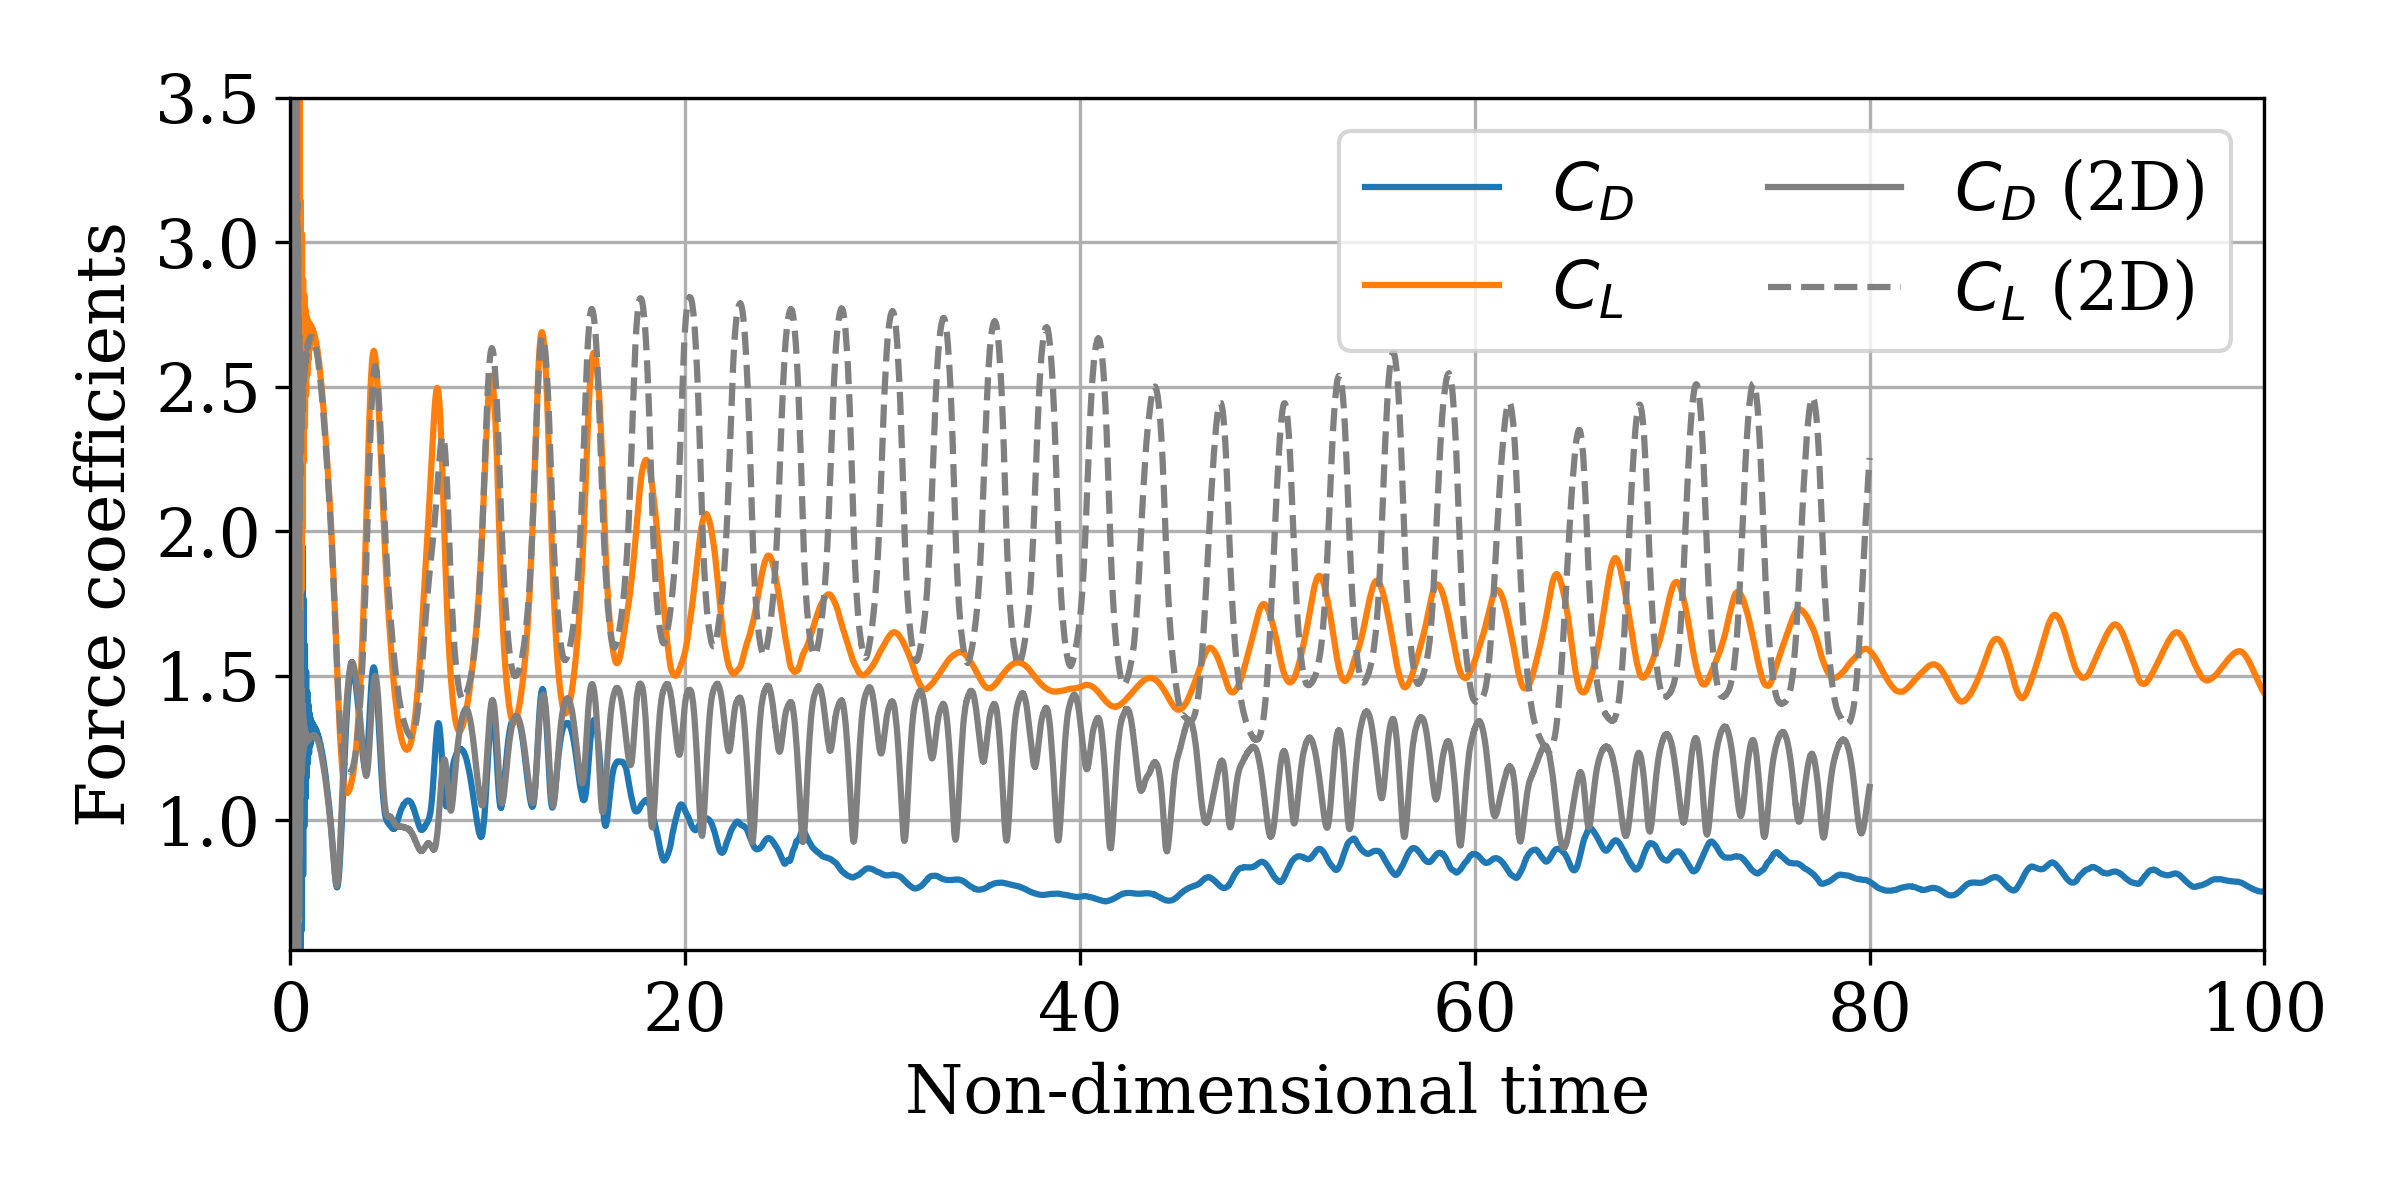
\includegraphics[width=7cm]{figures/forceCoefficientsCompare2D.png}
    \caption{History of the force coefficients obtained with two- and three-dimensional simulations at Reynolds number $2000$ for a snake cross-section with a $35$-degree angle of attack.}
    \label{fig:force_coefficients}
\end{figure}

\begin{table}[!t]
    \caption{Time-averaged force coefficients on the snake cross-section at Reynolds number 1000 and angle of attack $35^o$ for the two- and three-dimensional configurations. (We average the force coefficients between $40$ and $80$ time units of flow simulation.)}
    \label{tab:force_coefficients}
    \centering
    \begin{tabular}{ccll}
        \hline
        Case & Mesh size & $<C_D>$ & $<C_L>$ \\
        \hline
        3D & $1071 \times 1072 \times 40$ & $0.8390$ & $1.5972$ \\
        2D & $1704 \times 1706$ & $1.1567$ ($+37.9\%$) & $1.8279$ ($+14.4\%$) \\
        \hline
    \end{tabular}
\end{table}

% \section*{Acknowledgment}

\bibliographystyle{IEEEtran}
% argument is your BibTeX string definitions and bibliography database(s)
\bibliography{IEEEabrv,MesnardoBarba2019}
%
% <OR> manually copy in the resultant .bbl file
%\begin{thebibliography}{1}
%\bibitem
%\end{thebibliography}

\end{document}


